\begin{figure}[htbp]
\centering
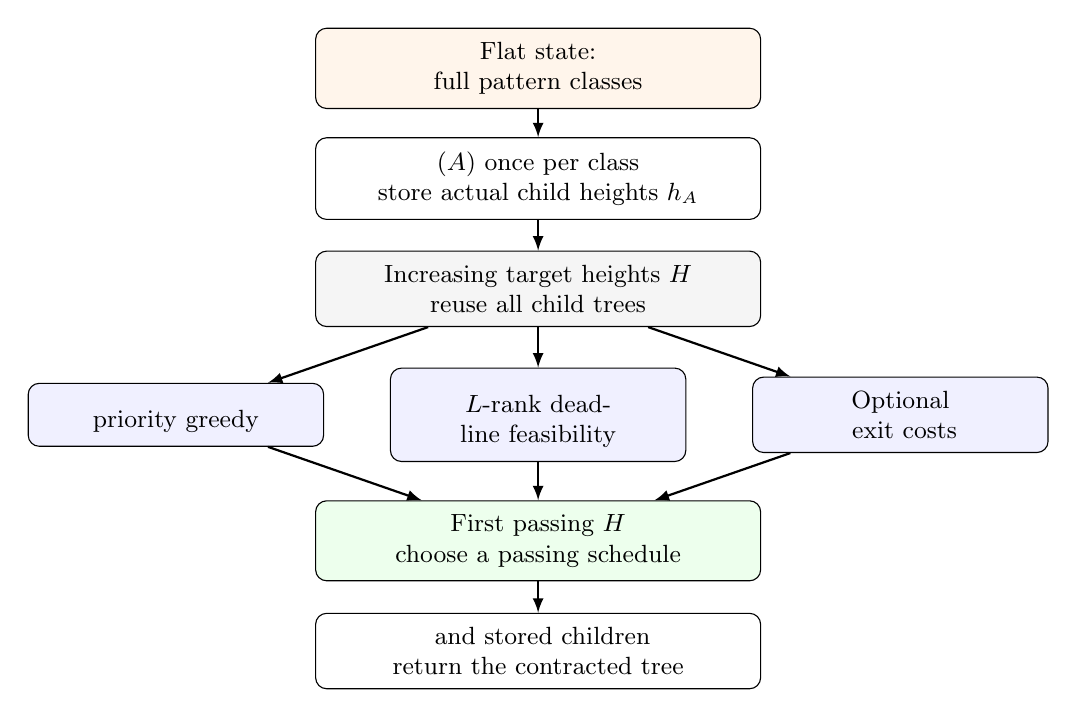
\begin{tikzpicture}[every node/.style={font=\small},
  box/.style={draw,rounded corners,align=center,inner sep=5pt,text width=3.4cm},
  wide/.style={box,text width=5.3cm},arr/.style={-latex,thick}]
  \node[wide,fill=orange!8] (hull) at (0,0)
    {Flat state: \HullData\\full pattern classes};
  \node[wide] (children) at (0,-1.4)
    {\HybridTree$(A)$ once per class\\store actual child heights $h_A$};
  \node[wide,fill=gray!8] (trial) at (0,-2.8)
    {Increasing target heights $H$\\reuse all child trees};
  \node[box,fill=blue!6] (priority) at (-4.6,-4.4)
    {\PriorityTrial\\priority greedy};
  \node[box,fill=blue!6] (slots) at (0,-4.4)
    {\SlotDP\\$L$-rank deadline feasibility};
  \node[box,fill=blue!6] (whole) at (4.6,-4.4)
    {Optional \SlotDP\\\EndpointCode\ exit costs};
  \node[wide,fill=green!7] (pass) at (0,-6)
    {First passing $H$\\choose a passing schedule};
  \node[wide] (attach) at (0,-7.4)
    {\EndpointCode\ and stored children\\return the contracted tree};
  \draw[arr] (hull) -- (children);
  \draw[arr] (children) -- (trial);
  \draw[arr] (trial) -- (priority);
  \draw[arr] (trial) -- (slots);
  \draw[arr] (trial) -- (whole);
  \draw[arr] (priority) -- (pass);
  \draw[arr] (slots) -- (pass);
  \draw[arr] (whole) -- (pass);
  \draw[arr] (pass) -- (attach);
\end{tikzpicture}
\caption{Construction of the polynomial maximum-depth tree at a flat
state. Arrows pass explicitly computed geometry, heights, or schedules.
The logarithmic cap $L$ is fixed at the original root. The priority
alternative guarantees that some height trial passes; the exact and
whole-exit alternatives can accept an earlier trial. The unknown optimum
is used only in the proof, never in this procedure.}
\label{fig:hybrid-procedure-flow}
\end{figure}

